\chapter{معماری مدل‌های ارائه شده}
\section{مدل‌های پایه مورد استفاده در تشخیص اخبار جعلی}
تاکنون در زبان فارسی، پژوهشگران عمدتاً از مدل‌های مرسوم یادگیری ماشین برای تشخیص اخبار جعلی استفاده کرده‌اند. یکی از اصلی‌ترین دلایل استفاده از این روش‌ها کافی نبودن داده‌های یادگیری برای آموزش مدل‌های به‌روز و پیچیده است. در این پروژه، پس از جمع‌آوری یک مجموعه داده از اخبار جعلی منتشرشده در پایگاه‌های خبری فارسی، استفاده از مدل‌های عمیق امکان‌پذیر می‌شود. به‌طورکلی پردازش داده متنی در سیستم تشخیص خبر جعلی‌ از دو بخش اصلی بازنمایی متن و دسته‌بندی متن تشکیل شده‌است که در ادامه توضیح هریک از آن‌ها ارائه می‌گردد.
\subsection{شبکه عصبی پرسپترون ساده}
شبکه عصبی شامل شبکه‌ای از عناصر پردازش ساده (نورون‌ها) است، که می‌تواند رفتار پیچیده کلی تعیین‌شده‌ای از ارتباط بین عناصر پردازش و پارامترهای عنصر را نمایش دهد. این نورون‌ها مجموعه‌ای از ویژگی‌های ورودی را گرفته و باتوجه‌به ماتریس وزن، تمایل\LTRfootnote{Bias} و «تابع فعال‌سازی»\LTRfootnote{Activation function} خروجی را به‌دست می‌آورد. \figurename~\ref{fig.slp} نمایی از شبکه عصبی ساده را نمایش می‌دهد.
\begin{figure}[!h]
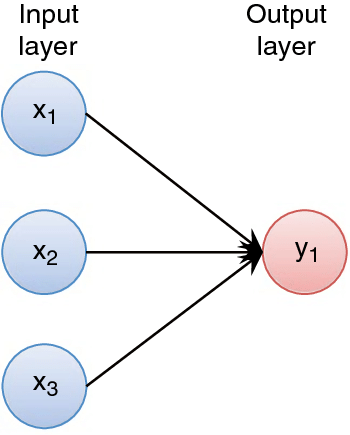
\includegraphics[width=0.25 \textwidth]{slp}
\centering
\caption{نمایی از شبکه عصبی دارای نورون‌های مدل پرسپترون ساده}
\label{fig.slp}
\end{figure}

\begin{table}[!h]
\caption{توابع فعال‌ساز پرکاربرد به‌همراه روابط و نمودار آنها}
\label{table:activationFunctions}
\begin{center}
\begin{tabular}{M{3cm}M{5cm}M{7cm}}
نام & نمودار & تعریف ریاضی \\
\hline
\hline
\lr{Binary step} &
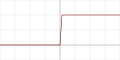
\includegraphics[scale=1]{binary_step} & 
\[f(x) =
\begin{cases}
1, & \verb|x| \geq \verb|0| \\
0, & \verb|x| < \verb|0| \\
\end{cases}
\] \\ \hline

\lr{Sigmoid} &
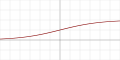
\includegraphics[scale=1]{sigmoid} & 
\[f(x) =
\frac{1}{1 +‌\exp(-x)}
\] \\ \hline

\lr{Tanh} &
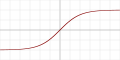
\includegraphics[scale=1]{tanh} & 
\[f(x) =
tanh(x) = \frac{\exp(x) - \exp(-x)}{\exp(x) +‌\exp(-x)}
\] \\ \hline

\lr{Relu} &
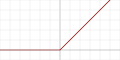
\includegraphics[scale=1]{relu} & 
\[f(x) =
\begin{cases}
x, & \verb|x| \geq \verb|0| \\
0, & \verb|x| < \verb|0| \\
\end{cases}
\] \\ \hline
\end{tabular}
\end{center}
\end{table}


توابع فعال‌ساز با استفاده از ایجاد روابط غیرخطی میان ورودی و خروجی هر نورون سعی می‌کند تا ارتباطات پیچیده‌تری را یاد بگیرد. در \tablename~\ref{table:activationFunctions} چند نمونه از این توابع فعال‌ساز با نمودار مربوط به آنها آورده شده‌است.


%==================================================================
\subsection{شبکه عصبی پیچشی}
این دسته از شبکه‌ها که در ابتدا برای حل مسائل بینایی ماشین ارائه شده بود با به‌کاربستن هسته‌هایی\LTRfootnote{Kernel} با وزن‌های مشترک روی ناحیه‌هایی از ورودی عمل پیچش را انجام می‌دهد. 

 ایده استفاده از وزن‌های‌ مشترک زمانی مطرح شد که تصاویر خاصیت ایستا دارد. این بدان معناست که آماره‌های بخش‌های مختلف یک تصویر و الگوی کلی آنچه که قرار است در تصویر تشخیص داده شود ثابت است و تغییری نمی‌کند.
 
  
 اما استفاده از شبکه‌های
 پیچشی تنها منحصر به حوزه پردازش تصویر نیست و به‌مرور وارد سایر حوزه‌ها نظیر پردازش متن نیز شده‌است.
 این نوع شبکه‌ها عمدتاً از لایه‌هایی مانند ادغام\LTRfootnote{Pool} و پیچش\LTRfootnote{Convolution} تشکیل شده‌است. لایه پیچش از فیلترهایی استفاده می‌کند که با
 انجام عملیات پیچش برروی داده ورودی، یک نگاشت ویژگی جدید تولید می‌کند. لایه ادغام نیز معمولاً پس از لایه پیچش،
 برای نمونه‌گیری از نگاشت ویژگی استفاده می‌کند. دو نوع پرکاربرد این نمونه‌گیری، «میانگین مقادیر»\LTRfootnote{Average pooling} و «بیشترین مقدار»\LTRfootnote{Max pooling} است. درنهایت پس‌از به‌دست‌آمدن نگاشت ویژگی نهایی و بردارسازی آن، از یک شبکه عصبی چند لایه استفاده می‌شود تا خروجی
 نهایی باتوجه‌به ورودی به‌دست آید. از شبکه‌های عصبی پیچشی دو بعدی، عمدتاً برای عکس و از شبکه‌های عصبی پیچشی یک
 بعدی بیشتر برای متن استفاده می‌شود. در \figurename~\ref{fig.alexnet} یک نمونه از شبکه عمیق پیچشی  که برای دسته‌بندی عکس استفاده شده می‌شود نشان داده شده‌است.

\begin{figure}[!h]
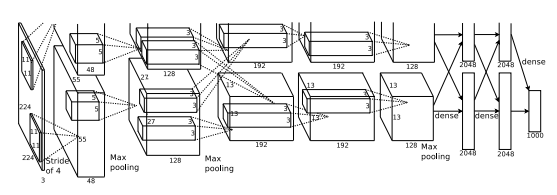
\includegraphics[width=1 \textwidth]{alexnet}
\centering
\caption{.نمای کلی مدل پیچشی الکس‌نت \citep{krizhevsky2012imagenet}}
\label{fig.alexnet}
\end{figure}

\vspace{3mm}

\begin{figure}[!h]
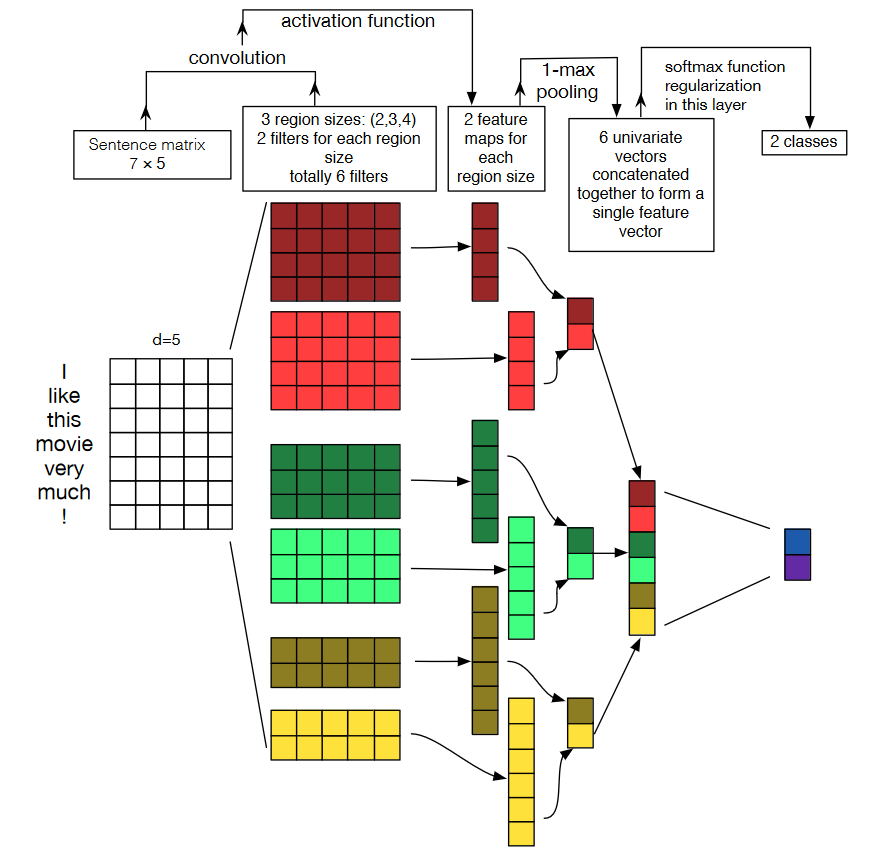
\includegraphics[width=0.85 \textwidth]{cnn}
\centering
\caption{نمای کلی یک شبکه عصبی عمیق پیچشی \citep{le2017convolutional}}
\label{fig.sentimentAnalyzing}
\end{figure}

در ادامه یک مثال کاربردی از شبکه پیچشی در زمینه پردازش متن توضیح داده می‌شود. \figurename~\ref{fig.sentimentAnalyzing} را درنظر بگیرید. یکی از مسائل  پرکاربرد در حوزه پردازش زبان طبیعی، «تحلیل احساسات»\LTRfootnote{Sentiment Analysis} است که در این مثال ما به‌طور خاص  به‌دنبال تشخیص احساس و تمایل در جمله \lr{I like this movie very much.} هستیم. در این مثال کاربردی، داده ورودی به جای یک تصویر، یک ورودی به ابعاد  $n \times d$  است که $n$ طول جمله بر حسب واژه‌ها و $d$ ابعاد تعبیه\LTRfootnote{Embedding} واژه‌ها می‌باشد. سپس در لایه پیچش، روی این ورودی هسته‌هایی با ابعاد مختلف حلقه‌ای زده می‌شود. معمولاً ابعاد این هسته‌ها برای متن ورودی یک بعدی است که این به‌معنای داشتن یک پنجره لغزان روی سطرهای ماتریس می‌باشد. به بیان دیگر، می‌توان این هسته‌ها را بازنمایی سطح بالا از چندتایی‌های واژه‌های ورودی دانست. در لایه بعد، ادغام بیشینه روی خروجی مرحله قبل  انجام شده و خروجی آنها نیز برای دسته‌بندی به لایه تماماً متصل داده می‌شود. در مسئله تحلیل احساس می‌توان فرض کرد که عبارت \lr{like this movie} (که مهم‌ترین عامل نشان‌دهنده احساس است)  در هر جای متن  به‌عنوان احساس مثبت درنظر گرفته شده و مکان این عبارت برای تصمیم‌گیری درمورد دسته‌بندی آن اهمیتی ندارد. بنابراین، با حرکت آن پنجره لغزان می‌توان عبارات مثبت را شناخت؛ و درنهایت می‌توان با استفاده از این اطلاعات، مثبت یا منفی بودن احساس کل عبارت را مشخص نمود.

%==================================================================

\section{مدل‌های بازنمائی متن مبتنی بر بافت}
اولین قدم برای پردازش متن، ایجاد بازنمایی مناسب برای متن ورودی است. در این بخش به بررسی مدل‌های زبانی برت \citep{devlin2018bert} و مدل‌های مبتنی بر معماری آن مانند برت چند زبانه \LTRfootnote{Multilingual BERT}، پارس‌برت \LTRfootnote{ParsBERT} \citep{ParsBERT}، آلبرت‌-فارسی \LTRfootnote{ALBERT-Persian} \citep{ALBERTPersian}، ایکس.ال.ام-روبرتا \LTRfootnote{XLM-RoBERTa} \citep{conneau2019unsupervised} می‌پردازیم.

\subsection{برت}
\label{section.bert}
\citet{devlin2018bert} 
یک مدل زبانی جدید با نام برت را معرفی کردند. ایده اصلی این مدل استفاده از انتقال‌دهنده‌های‌\LTRfootnote{Transformer} دوطرفه برای یادگیری معنا و ساختار واژه‌های موجود در متن است. مدل برت به‌صورت دو نسخه «برت پایه»\LTRfootnote{BERT-Base} و «برت بزرگ»\LTRfootnote{BERT-Large} معرفی شده‌است. برت پایه دارای 12 لایه انتقال‌دهنده و  110 میلیون پارامتر و برت بزرگ دارای  24 لایه و 340 میلیون پارامتر است. انتقال‌دهنده‌ها از «مکانیزم توجه»\LTRfootnote{Attention mechanism} در فرایند یادگیری استفاده می‌کند و سعی می‌کند تا ارتباط مفهومی میان واژه‌های موجود در یک جمله را به‌درستی یاد بگیرد. فرایند یادگیری مدل‌های زبانی عموماً به این صورت است که تلاش می‌کند تا واژه بعدی یک دنباله را حدس بزند و بر این اساس، ارتباط میان واژه‌ها را تشخیص دهند. اما در مدل زبانی برت که به‌صورت دوطرفه (چپ‌به‌راست و راست‌به‌چپ) متن را بررسی می‌کند نمی‌توان فقط از این روش استفاده کرد. برای آموزش مدل برت دو مرحله زیر برروی پیکره‌های متنی ویکی‌پدیا و کتاب‌ها اعمال شده‌است. 
 در \figurename~\ref{fig.BERT} نحوه آموزش در مدل برت نمایش داده شده‌است.

\begin{figure}[!h]
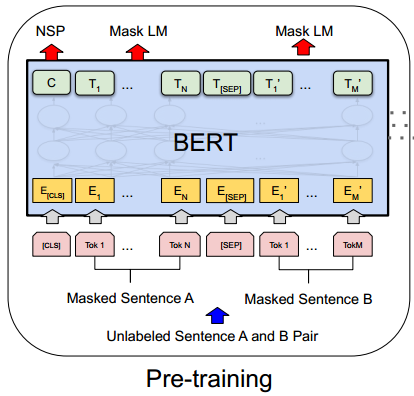
\includegraphics[width=0.6 \textwidth]{bert}
\centering
\caption{ نحوه عملکرد یادگیری مدل برت \citep{devlin2018bert}}
\label{fig.BERT}
\end{figure}

\begin{itemize}
\item \textbf{پوشش واژه‌ها} \\
قبل از استفاده از داده‌ها در شروع فرایند یادگیری، 15 درصد از واژه‌های داخل متن به‌صورت تصادفی انتخاب می‌شود. 
 از این حجم واژه‌ها 80‌ درصد واژه‌ها با عبارت \verb|[MASK]| جایگزین شده و 10 درصد با یک واژه تصادفی جایگزین می‌شود و 10
 درصد دیگر بدون تغییر باقی می‌ماند. در ادامه، مدل سعی می‌کند تا با استفاده از اطلاعات زمینه‌ای، این واژه‌ها را حدس بزند.
 این کار با اضافه‌کردن یک لایه پس از لایه کدگذار مدل برت انجام می‌شود تا با استفاده از آن، احتمال وجود هریک از واژه‌ها
 مشخص شود و با داشتن واژه اصلی، خطای مدل حساب شده و تمامی وزن‌ها به‌روزرسانی می‌شود.

\item \textbf{پیش‌بینی جمله بعدی} \\
در این حالت، مدل برت یک جفت دنباله مانند آ و ب را دریافت می‌کند. در ابتدا و انتها جملات عبارات \verb|[CLS]| و \verb|[SEP]| قرار
 می‌گیرد. پس از اضافه‌کردن نوع جمله ($آ$ یا $ب$) به ویژگی‌های نهفته هر جمله، تمامی ورودی‌ها وارد انتقال‌دهنده‌ها شده و
 درنهایت با استفاده از یک لایه، مقدار احتمال ظهور دنباله $ب$ به‌عنوان جمله بعدی دنباله $آ$ مشخص می‌شود. با این روش مدل برت
 تلاش می‌کند تا مفاهیم زمینه‌ای را به‌طور کامل میان واژه‌ها و عبارات یاد بگیرد.
\end{itemize}

درنهایت پس از آماده‌شدن مدل زبانی، می‌توانیم از آن در مسائل مختلف مانند دسته‌بندی متن، پرسش و پاسخ\LTRfootnote{Question Answering (QA)} و تشخیص
 موجودیت‌های نامدار\LTRfootnote{Name Entity Recognition (NER)} استفاده کنیم.


\subsection{برت چند زبانه}
	مدل زبانی برت چند زبانه \citep{devlin2018bert} با استفاده از داده‌هایی از ۱۰۴ زبان مختلف شامل زبان فارسی آموزش داده شده‌است. مدل زبانی برت دارای دو نوع پایه و بزرگ است که ما در این پروژه از مدل برت پایه، شامل ۱۲ لایه انتقال‌دهنده و ۱۱۰ میلیون پارامتر استفاده کرده‌ایم. این مدل با استفاده از پیکره متنی ویکی‌پدیا\LTRfootnote{Wikipedia} که به زبان‌های مختلف موجود است، آموزش داده شده‌است. 
	
\subsection{پارس‌برت}
	\cite{ParsBERT}
	مدل زبانی پارس‌برت که مبتنی بر معماری مدل برت است،انحصاراً برای زبان فارسی آموزش داده شده‌است. این مدل عملکرد بهتری نسبت‌به مدل‌های چند زبانی مانند برت داشته‌است. همچنین به‌دلیل آنکه این مدل تنها برای زبان فارسی ارائه شده‌است، سبک‌تر از مدل زبانی برت چندزبانه است. به‌منظور آموزش مدل‌زبانی پارس‌برت از منابع متنی موجود در وب‌سایت‌های ویکی‌پدیا، بیگ‌بنگ، چطور، الی گشت، دیجی کالا، تد تاک، کتاب‌ها و پیکره میراث استفاده شده‌است. همچنین برای ارزیابی مدل‌ ارائه‌شده در پارس‌برت از تحلیل احساسات، تشخیص موجودیت‌های نامدار و دسته‌بندی متن استفاده شده‌است.
	
\subsection{آلبرت-فارسی}
	مدل‌زبانی آلبرت یک نسخه سبک‌تر از برت است که معماری کاملاً مشابه‌ای با آن دارد که در پیاده‌سازی آن تغییر اندکی نسبت‌به مدل برت وجود دارد \citep{ALBERTPersian}. آلبرت-فارسی، مانند مدل‌زبانی پارس‌برت بر روی  پیکره‌های متنی فارسی آموزش داده شده‌است. علیرغم اینکه منابع این پیکره‌های فارسی مشابه مدل‌زبانی پارس‌برت است، به‌مراتب حجم  کمتری نسبت‌به پارس‌برت دارد.
	
\subsection{ایکس.ال.ام-روبرتا}
	با توجه به موفقیت‌های چشمگیر مدل‌های ازپیش آموزش‌دیده، \cite{conneau2019unsupervised} یک مدل‌ بین‌زبانی ارائه کردند که توانست دقت بهتری را در مقایسه با مدل‌های زبانی رایج مانند برت ثبت کند. این مدل که برروی دادگان ۱۰۰ زبان مختلف ازجمله فارسی آموزش داده شده‌است  با استفاده از ۳ روش آموزش داده می‌شود: (۱) پیش‌بینی کلمه بعدی، (۲) پیش‌بینی کلمه پوشیده شده و (۳) مدل زبانی مبتنی بر ترجمه.
%==================================================================

\section{معماری‌های پیشنهادی برای تشخیص اخبار جعلی}
به‌طور کلی، بازنمایی حاصل از برت به دو صورت مختلف می‌تواند مورد استفاده قرار بگیرد.
\begin{itemize}
\item بازنمایی تجمعی\LTRfootnote{Pooled} به ازای هر دنباله از واژه‌های ورودی، یک بازنمایی کلی برای کل دنباله ارائه می‌کند.
\item بازنمایی دنباله‌ای\LTRfootnote{Sequence} که در آن برای هر واژه یک بردار بازنمایی مبتنی‌بر بافت ارائه
 می‌گردد.
\end{itemize}

\noindent
در این پروژه، رویکرد پیشنهادی دو معماری مختلف مورد استفاده قرار گرفته‌است که در هر یک از این معماری‌ها، یکی از دو حالت فوق به‌کار رفته‌است.  در روش اول که آن را روش «برت+پرسپترون ساده» می‌نامیم، بازنمایی حالت دوم که یک بازنمایی یکتا برای هر جمله/عبارت ارائه می‌گردد به‌کار گرفته می‌شود. و در روش دوم که آن را مدل «برت + پیچشی» می‌نامیم، بازنمایی حالت اول که براساس تفکیک واژه‌ها ایجاد می‌شود به‌کار می‌رود.


%==================================================================

\subsection{مدل زبانی مبتنی بر بافت + پرسپترون ساده}
برای استفاده از مدل‌‌های مبتنی بر معماری ‌برت در مسئله دسته‌بندی کافی است تا از بردار خروجی متناظر با توکن \verb|[CLS]| به‌عنوان بردار نماینده آن دنباله استفاده کنیم. دلیل استفاده از این بردار این است که شامل تمامی بردارهای توکن‌های موجود در متن است، درحالی‌که بردارهای متناظر با توکن‌های دیگر تنها نماینده آن توکن در عبارت ورودی است. بنابراین کافی است تا بردار نماینده دنباله متنی ورودی را وارد یک لایه تکی پرسپترون کنیم که می‌تواند عمل تشخیص برچسب دنباله ورودی را برای ما انجام دهد. این مدل در \figurename~\ref{fig.bertSLP} ترسیم شده‌است.

به عبارت دیگر، با استفاده از بازنمایی به‌دست‌آمده از مدل برت برای یک جمله و داشتن برچسب آن سعی می‌کنیم تا با استفاده از  دادگان موجود، یک مدل کامل برای تشخیص اخبار جعلی بسازیم. برای این هدف کافی است تا وزن‌های ورودی به لایه پرسپترون  ساده آموزش داده شود به صورتی که بتواند اخبار را به درستی دسته‌بندی کند. 

\begin{figure}[!h]
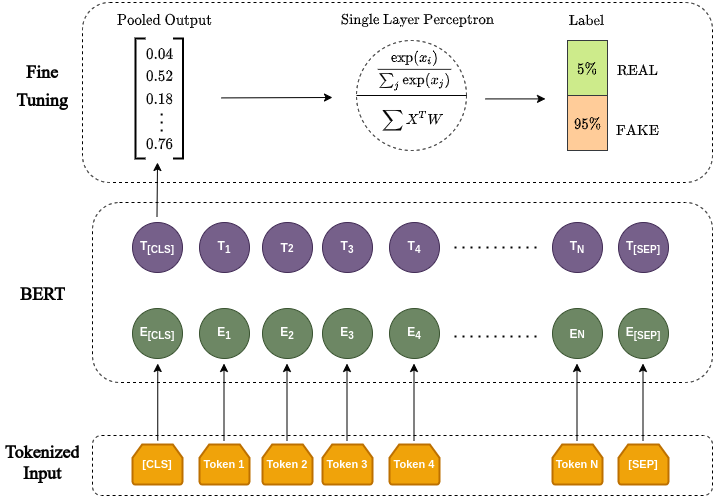
\includegraphics[width=0.75 \textwidth]{bert_slp}
\centering
\caption{نحوه استفاده از یک لایه پرسپترون ساده درکنار مدل برت}
\label{fig.bertSLP}
\end{figure}
\noindent

به‌منظور جلوگیری از بیش‌برازش\LTRfootnote{Overfitting} شدن مدل، از روش «حذف تصادفی نورون‌ها»\LTRfootnote{Dropout} استفاده می‌کنیم تا مدل نهایی تا حد ممکن ساده باشد و به‌درستی ویژگی‌های مهم را یاد بگیرد. در انتهایی‌ترین بخش مدل هم یک لایه نورون به تعداد دسته‌های دادگان ورودی وجود دارد که تابع فعال‌ساز آنها بیشینه هموار است. چرا که نیاز داریم تا احتمال تعلق‌داشتن خبر به هر دسته را بدانیم و بیشترین آن را به‌عنوان برچسب پیشبینی‌شده اعلام نماییم.

تابع «خطا آنتروپی متقاطع طبقه‌ای»\LTRfootnote{ Categorical Cross-entropy} نیز برای محاسبه میزان خطای پیش‌بینی مدل دسته‌بند خبر جعلی استفاده شده‌است که رابطه ریاضی آن در زیر آمده‌است.

\begin{equation}
Loss = - \sum_{c=1}^{M}y_{o,c} . log(p_{o,c})
\end{equation}
در این رابطه، $M$ تعداد دسته‌ها و $y_o$ بردار تک‌روشن از برچسب خبر $o$ است و $p_o$ نیز بردار احتمال پیش‌بینی‌شده توسط مدل است که نشان‌دهنده احتمال تعلق به هر دسته است.

%==================================================================

\subsection{مدل زبانی مبتنی بر بافت + پیچشی}
این مدل از بازنمایی که توسط یک مدل‌زبانی مبتنی بر برت برای واژه‌های یک جمله تولید شده‌است، استفاده می‌کند تا با استفاده از یک لایه شبکه عصبی پیچشی، عملیات نگاشت ویژگی را انجام دهد. پس‌از عملیات یادگیری، این مدل سعی می‌کند تا با تبدیل بازنمایی تولیدشده به یک بازنمایی دیگر، عملیات پیش‌بینی کذب‌بودن یا اصیل‌بودن یک خبر را انجام دهد. در این مدل، به‌جای بردار خروجی تجمیعی، از بردار خروجی دنباله‌ای که شامل دنباله‌ای از بردارهای تک‌تک واژه‌های داخل خبر است استفاده می‌گردد؛ چراکه با استفاده از لایه‌های پیچشیِ پس‌از آن می‌توان همنشینی‌هایی از واژه‌ها که نشان‌دهنده اخبار جعلی است را شناسایی کرد. برای این منظور، از یک لایه پیچشی یک‌بُعدی با تعداد ۲۰۴۸ فیلتر و هسته‌هایی به اندازه ۴ استفاده می‌کنیم. همچنین تابع فعال‌ساز این لایه، تابع «یک‌سوساز خطی»\LTRfootnote{ReLU} است. پس از این لایه، یک لایه ادغامِ بیشترین مقدار با اندازه ۴ قرار دارد. درنهایت، با استفاده از یک «لایه تخت‌شونده»\LTRfootnote{Flatten layer}، ماتریس مرحله قبل به یک بردار یک بعدی تبدیل می‌شود تا با استفاده از یک لایه چگال\LTRfootnote{Dense} با استفاده از تابع فعال‌ساز «بیشینه هموار»\LTRfootnote{Softmax}، احتمال هر دسته مشخص شود. \figurename~\ref{fig.bertCNN} نحوه اتصالات و به‌دست‌آوردن ویژگی‌های سطح بالاتر را نشان می‌دهد.

\begin{figure}[!h]
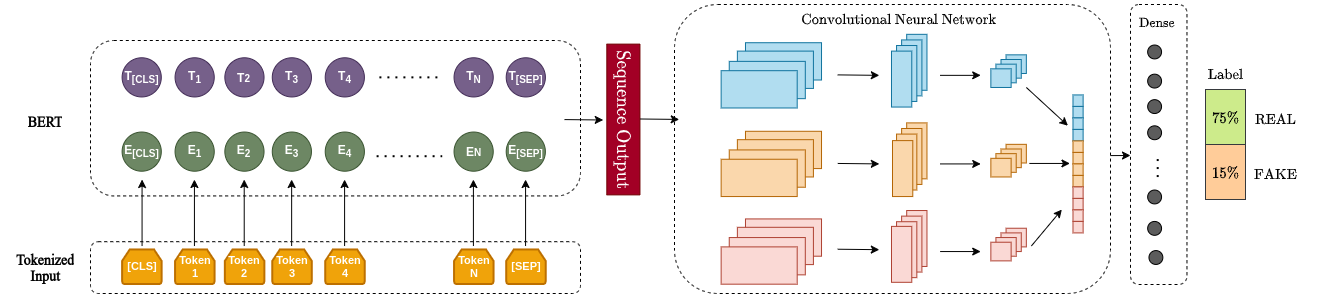
\includegraphics[width=1 \textwidth]{bert_cnn}
\centering
\caption{نحوه ارتباط لایه پیچشی با بردارهای خروجی مدل برت}
\label{fig.bertCNN}
\end{figure}
